\chapter{Material und Methoden}\label{mat_and_method}
\section{Material}\label{material}
Als Stichprobe stehen die Datensätze von insgesamt 86 Patient*innen zur Verfügung. Bereitgestellt wurden die Datensätze an Patient*innen vom \textbf{Universitätsklinikum Regensburg}. Die dazugehörigen Grade der House-Brackmann Skala sind hierbei innerhalb der Stichprobe allerdings nicht gleichverteilt vorhanden. Der Grad VI ist prozentual ungefähr im gleichen Maße vorhanden wie die Grade I-V zusammen (siehe Abb. \ref{cap:pie_grade}). Der Grad I ist nur mit eine*r Patient*in vertreten. Diese ungleiche Verteilung wird bei der späteren Auswirkung berücksichtigt werden.

\begin{figure}[!b]\centering
\begin{tikzpicture}
\pie[sum=auto, radius=2.7, text=pin]{1/I , 6/II, 9/III, 22/IV, 8/V, 40/VI }
%\pie[pos ={10,0}, sum=auto, radius=3.5, text=legend]{1/I , 6/II, 9/III, 22/IV, 8/V, 40/VI }
\end{tikzpicture}
\caption[Verteilung der einzelnen Grade der House-Brackmann Skala]{Verteilung der einzelnen Grade der House-Brackmann Skala des zu Verfügung stehenden Datensatzes. Klar erkennbar ist das ungleiche Vorhandensein der Grade.}\label{cap:pie_grade}
\end{figure}\label{fig:pie_grade}


Jeder Datensatz jede*r Patient*in besteht aus neun verschiedenen Bildern, die verschiedene Posen darstellen. Die Gesichtsausdrücke in den Einzelbildern können jeweils einem konkreten Teil des House-Brackmann Scores zugeordnet werden. Zudem werden die normalerweise in Bewegung stattfindenden Ausdrücke statisch im Bild eingefangen.

\clearpage

Die Bildcodierung (Posendarstellung) dieser neun Bilder lautet:

\begin{enumerate}
  \setlength\itemsep{-0.6em}
\item Ruhender Gesichtsausdruck
\item Augenbrauen Heben
\item Lächeln, geschlossener Mund
\item Lächeln, geöffneter Mund
\item Lippen Schürzen, \glqq Duckface\grqq{}
\item Augenschluss, leicht
\item Augenschluss, forciert
\item Nase Rümpfen
\item Depression Unterlippe
\end{enumerate}

Das Bild mit der Codierung 1 fokussiert sich dabei auf die Symmetrie in Ruhe. Die zweite Pose 2 bildet die Stirn ab. Dadurch sollen die Auswirkungen sowie die Beweglichkeit der Muskeln rund um die Stirnpartie bildlich festgehalten werden (absichtliche Faltenbildung). Der Lidschluss wird mit den Bildern 6 und 7 statisch eingefangen. Ein nicht geschlossenes Auge wird durch das Weiß des Augapfels für das System erkennbar. Die Gesichtsausdrücke auf den Bildern 3, 4, 5, 8 und 9 zeigen den Mund in unterschiedlichen Positionen. So sollen die Unterschiede zwischen den beiden Gesichtshälften am besten aufgezeigt werden. Die Posen für den Mund sind von außen betrachtet einer der Hauptmerkmale für eine Fazialisparese, welche auch schon für einen Laien erkennbar ist.

Problematisch dabei ist, dass nicht für jede*n Patient*in alle neun korrespondierenden Bilder vorhanden sind. Besonders ist dies bei den Bildcodierungen 5, 7, 8 und 9 der Fall (siehe Abb. \ref{cap:bar_code}). Beim Trainieren der Neuronalen Netze ist darauf Rücksicht zu nehmen.


\begin{figure}[!tb]\centering
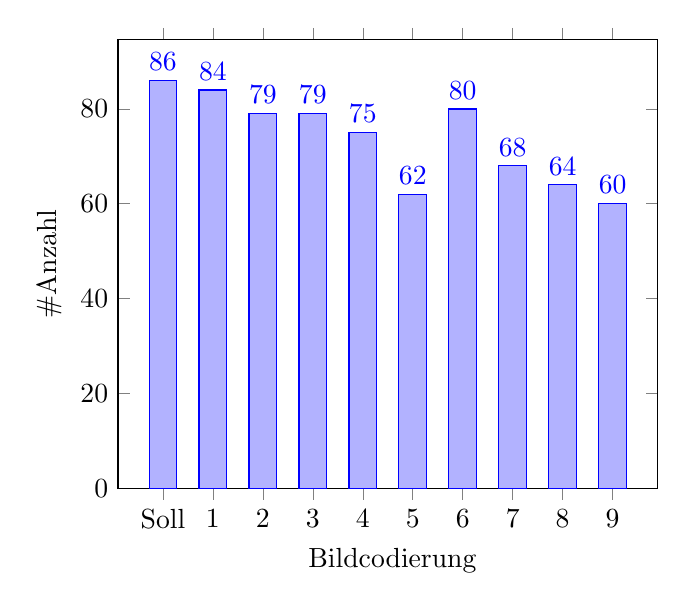
\begin{tikzpicture}
\begin{axis}
[
    ybar,
    ymin=0,
    %enlargelimits=0.15,
    ylabel={\#Anzahl}, % the ylabel must precede a # symbol.
    xlabel={\ Bildcodierung},
    symbolic x coords={Soll, 1, 2, 3, 4, 5, 6, 7, 8, 9},
    xtick=data,
    nodes near coords, % this command is used to mention the y-axis points on the top of the particular bar.
    nodes near coords align={vertical},
    ]
\addplot coordinates {(Soll,86) (1,84) (2,79) (3,79) (4,75)
                      (5,62)    (6,80) (7,68) (8,64) (9,60) };

\end{axis}
\end{tikzpicture}
\caption[Anzahl der vorhandenen  Einzelbilder aller Patient*innen]{Anzahl der vorhandenen  Einzelbilder aller Patient*innen. Der Sollwert beträgt 86 für alle Bildcodierungen.}\label{cap:bar_code}
\end{figure}\label{fig:bar_code}





\clearpage
\section{Methode}\label{method}
\subsection{Module}\label{module} %Modulverarbeitung
Für die Detektion des Grades nach House-Brackmann werden die einzelnen Merkmale der Skala in Module eingeteilt (siehe Abb. \ref{cap:module_graph}). Ziel dieser Aufteilung ist es, Expertensysteme für die Teilbereiche der House-Brackmann Skala zu bilden. Diese müssen für die Detektion angepasst werden. Die dynamischen Eigenschaften Stirn, Lidschluss und Mund können so nicht als ein Label interpretiert werden. Die neun Eingabebilder für das System stellen die Posen statisch dar. So können alle Eigenschaften bis auf Lidschluss nach der House-Brackmann Skala auf die Grundlabel \glqq Normal\grqq{}, \glqq minimale Asymmetrie\grqq{}, \glqq Asymmetrie\grqq{} und \glqq Keine\grqq{} aufgeteilt werden. Bei Lidschluss kommen stattdessen nur die zwei Möglichkeiten \glqq vollständig geschlossen\grqq{} oder \glqq geöffnet\grqq{} infrage (siehe Tabelle \ref{cap:housebrackmannnew}).
Nach dieser Tabelle werden so für die einzelnen Module die passenden Label bestimmt. Die Spalten entsprechen dabei den einzelnen Modulen. Die Überschrift der Spalte bezeichnet das einzelne Modul. Der Inhalt dieser sind die zu ermittelnden Klassen für das Modul numemriert von 0 beginnend.

\begin{table}[h]\vspace{1ex}\centering
  \begin{tabular}{c||c|c|c|c|}
  Grad & Symmetrie    & Stirn  & Lidschluss    & Mund         \\ \hline\hline
  I    & Normal       & Normal & Vollständig   & Normal       \\ \hline
  II  & Normal & Normal                                                        & Vollständig & \begin{tabular}[c]{@{}c@{}}minimale\\ Asymmetrie\end{tabular} \\ \hline
  III & Normal & \begin{tabular}[c]{@{}c@{}}minimale\\ Asymmetrie\end{tabular} & Vollständig & \begin{tabular}[c]{@{}c@{}}minimale\\ Asymmetrie\end{tabular} \\ \hline
  IV   & Normal       & Keine  & Unvollständig & Asymmetrisch \\ \hline
  V    & Asymmetrisch & Keine  & Unvollständig & Asymmetrisch \\ \hline
  VI   & Keine        & Keine  & Unvollständig & Keine        \\ \hline
  \end{tabular}
  \caption[Angepasste House-Brackmann Tabelle zur Bestimmung der Label/Klassen]{Angepasste House-Brackmann Tabelle zur Bestimmung der Label/Klassen aus der Originaltabelle \ref{cap:housebrackmann} (eigene entwickelte Interpretation)}\label{cap:housebrackmannnew}
\vspace{2ex}\end{table}\label{table:housebrackmannnew}



\begin{figure}[!tb]\centering
\begin{tikzpicture}[->,>=stealth',shorten >=1pt,auto,node distance=2.5cm,semithick]
  \tikzstyle{every state}=[fill=cyan,draw=black,text=black]

  \tikzstyle{level1} = [rectangle, draw, fill=green!40!blue!20, text width=8cm, text centered, inner sep=1pt  , minimum height=1.3cm]
  \tikzstyle{level2} = [rectangle, draw, fill=blue!20,          text width=2.4cm, text centered, rounded corners, minimum height=4cm]
  \tikzstyle{level3} = [rectangle, draw, fill=green!40!blue!20, text width=8cm, text centered, inner sep=1pt  , minimum height=1.3cm]
  \tikzstyle{level4} = [rectangle, draw=white, fill=white, text width=1cm, text centered, minimum height=0.1cm, minimum width=0.1cm]

  \tikzstyle{container} = [draw, rectangle, dashed, inner sep=8pt, minimum width=15cm]

  \node[level4]         (Z1)                                 {};

  \node[level1]         (A) [left of=Z1, xshift=8cm]        {Regions of Interest};
  \node[level2]         (B) [below left  of=A, yshift=-2cm] {Lidschluss \\$y_l \in [vollständig,\linebreak unvollständig]$};
  \node[level2]         (C) [below right of=A, yshift=-2cm] {Mund \\$y_m \in [normal,\linebreak minasymm,\linebreak asymm,\linebreak keine]$};
  \node[level2]         (D) [left  of=B, xshift=-1cm]       {Symmetrie \\$y_s \in [normal,\linebreak asymm,\linebreak keine]$};
  \node[level2]         (E) [right of=C, xshift=1cm]        {Stirn \\$y_f \in [normal,\linebreak minasymm,\linebreak keine]$};
  \node[level3]         (F) [below right of=B, yshift=-2cm] {Fusionierung};
  \node[container, fit=(B) (C) (D) (E)] (his) {};
    \node at (his.north west) [above right,node distance=0 and 0] {Module};

  \node[level4]         (Z2) [right of=F, xshift=3cm]        {};

  \path (Z1) edge [out=0   , in=180] node [left, xshift=-0.3cm, align=right]                {Input \\ Bilder $x_1 ... x_9$} (A)

        (A) edge [out=-145, in=90 ] node [right, yshift=-0.1cm, xshift=0cm   ] {$x_{l}$} (B) %Lidschluss
            edge [out=-35 , in=90 ] node [left , yshift=-0.1cm, xshift=0cm   ] {$x_{m}$} (C) %Mund
            edge [out=-160, in=90 ] node [above, yshift=-0.5cm, xshift=0.8cm ] {$x_{s}$} (D) %Symmetrie
            edge [out=-20 , in=90 ] node [above, yshift=-0.5cm, xshift=-0.5cm] {$x_{f}$} (E) %Stirn
        (B) edge [out=-90 , in=145] node [right, yshift=0.1cm , xshift=0cm   ] {$y_{l}$} (F)
        (C) edge [out=-90 , in=35 ] node [left , yshift=0.1cm , xshift=0cm   ] {$y_{m}$} (F)
        (D) edge [out=-90 , in=160] node [below, yshift=0.5cm , xshift=0.8cm ] {$y_{s}$} (F)
        (E) edge [out=-90 , in=20 ] node [below, yshift=0.5cm , xshift=-0.5cm] {$y_{f}$} (F)

        (F) edge [out=0   , in=180] node [right, xshift=0.3cm, align=left]                {Output \\ H-B Grad $[I, ..., VI]$} (Z2);

\end{tikzpicture}
\caption[Darstellung der Modulbauweise]{{Schematische Darstellung der Module. Die Eingabebilder $x_1, ..., x_9$ werden für jedes Bild in die Regions of Interest zerschnitten. Diese wandern als Stack $x_s, x_l, x_m, x_f$ (zerschnittenes Bildmaterial) in die einzelnen vorgesehenen Module. Danach werden diese zum \ac{hb_grade} fusioniert.}\label{cap:module_graph}}
\end{figure}\label{fig:module_graph}

Anhand von Markerpunkten im Gesicht der Patient*innen werden die neun Bilder jede*r Patient*in in die Bestandteile der Skala, die Regions of Interest, aufgeteilt. Dabei werden nur die relevanten Teile betrachtet, um proaktiv zu verhindern, dass die Neuronalen Netze nicht notwendige Eigenschaften als relevante Merkmale interpretieren. Zu den nicht notwendigen Bestandteilen der Bilder zählen der Hintergrund, welcher verschiedene Farben und Helligkeitsstufen annehmen kann, und der Körper der Patient*innen ab dem Kinn abwärts. Nur der Kopf wird für die Feststellung der Parese benötigt. Die Landmarks, die für die Einteilung in die Regionen verantwortlich sind, müssen sich hierfür immer an derselben Position $P$ im generierten Array befinden (siehe Abb. \ref{cap:r_of_interest}). Jedem Modul können so die relevanten Punkte (siehe Tabelle \ref{cap:rel_landmarks}) für ihr Modul sowie das Ausgabearray, welches die neun Bildausschnitte beinhaltet, zugeordnet werden. Für die Berechnung der neuen Eckpunkte für den Bildausschnitt werden die zugeordneten Landmarks $P$ in die nachfolgenden Formeln eingesetzt \cite{s151026756}:

\noindent\begin{minipage}{.5\linewidth}
\begin{alignat*}{3}
  a_{min} &= min(P[:, 0]) &\quad &\textrm{| Extrema links}\\
  a_{max} &= max(P[:, 0]) &\quad &\textrm{| Extrema rechts}\\
  b_{min} &= min(P[:, 1]) &\quad &\textrm{| Extrema oben}\\
  b_{max} &= max(P[:, 1]) &\quad &\textrm{| Extrema unten}
\end{alignat*}
\end{minipage}%
\begin{minipage}{.5\linewidth}
  \begin{equation}
  \begin{split}
    &\textrm{Zu erfüllende Bedingungen:}\\
    &\textrm{1.}\quad  a_{min} < a_{max}\\
    &\textrm{2.}\quad  b_{min} < b_{max}\\
    &\textrm{3.}\quad a_{min}, a_{max}, b_{min}, b_{max} \in \mathbb{N}
  \end{split}
  \label{eg:bbox}
  \end{equation}
\end{minipage}

\vspace{0.3cm}

\begin{table}[b]\vspace{1ex}\centering
\begin{tabular}{c||c|c|}
Modul & \begin{tabular}[c]{@{}c@{}}zugeschnittene\\ Eingabebilder als\\ Stack\end{tabular} & \begin{tabular}[c]{@{}c@{}}Betrachtete\\ Landmarks\end{tabular} \\ \hline\hline
Symmetrie  & $x_s$  & P(00) - P(68)  \\ %\hline
Lidschluss & $x_l$  & P(38) - P(47) \\ %\hline
Mund       & $x_m$  & P(48) - P(68) \\ %\hline
Stirn      & $x_f$  & P(17) - P(26) \\ \hline
\end{tabular}
\caption[Zuordnung der Module zu dem relevanten Punkten der Landmarks und das Eingabebild in die Module nach dem Ausschneiden vom Originalbild $x$]{Zuordnung der Module zu den relevanten Punkten der Landmarks und die Eingabebilder in die Module nach dem Ausschneiden vom Originalbild $x$}\label{cap:rel_landmarks}
\vspace{1ex}\end{table}\label{fig:rel_landmarks}


Dabei entsprechen ($a_{min}, b_{min}$), ($a_{min}, b_{max}$), ($a_{max}, b_{min}$) und ($a_{max}, b_{max}$) den vier neuen Ecken des benötigten Bildfragments. Die Ecken spannen ein Rechteck auf, dessen Inhalt als Eingabebild für eines der Module (z. B. Lidschluss nur Punkte $P(36)$ bis $P(47)$) relevant ist. Alles was sich nicht innerhalb des Rechteckes befindet, wird weggeschnitten. Ein Offset wird dazu noch in alle Richtungen addiert bzw. subtrahiert, um Ungleichheiten in der Landmarkberechnung auszugleichen, falls die Kontur nicht korrekt getroffen wurde. Wenn neun Bildfragmente für eines der Module berechnet worden sind, werden diese als Stack in die nächsttiefere Schicht weitertransportiert.

\begin{figure}[!t]\centering
%\resizebox{1.2\textwidth}{!}{
  %width=0.98\textwidth
\vspace{-1.3cm}
\makebox[0pt]{\includesvg[inkscapelatex=false, width=30cm]{./images/landmarks}}
%}
\vspace{-1cm}
\caption[Anschauliche Darstellung der Regions of Interest]{Anschauliche Darstellung der Regions of Interest. Inhalt des roten Rahmens ist die Eingabe für das Modul Symmetrie, grün für die Stirn, gelb der Lidschluss und pink für den Mund. Aus Datenschutzgründen durch einen Sobel-Filter verändert.}\label{cap:r_of_interest}
\end{figure}\label{fig:r_of_interest}


Die einzelnen Module Symmetrie, Lidschluss, Mund und Stirn (siehe Abb. \ref{cap:module_graph}) sind vortrainierte ResNet18 Netze vom ImageNet Contest. Benutzen von vortrainierten Netzen spart Trainingszeit an den Layern durch die schon vorhandenen angepassent Parametern vom ImageNet Contest. Die einzelnen Gewichte an den Kanten müssen so nur noch verfeinert werden, um das gewünschte Ergebnis zu erzielen. Für alle Experimente (siehe Kapitel \ref{experiment}) ist das gewählte Netz aus Gründen der Vergleichbarkeit der Ergebnisse identisch. Die Abbildungsvorschrift für die Relation Eingabebild $x$ mit der Pixelgröße $a, b$ und drei Schichten für den Farbraum RGB (bei Konkatenation vielfaches von 3) zu auszugebenden Wahrscheinlichkeiten der Klassen $y$ mit der Klassenlänge $k$ ist:

\vspace{-0.6cm}
\begin{equation}
y: \mathbb{R}^{3 \times a \times b} \to \mathbb{R}^{k}, y(x) = resnet18(x)
\label{eq:resnet}
\end{equation}

Jedem Eingabebild ist eine natürliche Zahl zugeordnet, die innerhalb der Trainingsphase und der Evaluierungsphase zu ermitteln ist. Diese Zahl ist letztendlich eine
Nummer, die ein Label/Klasse nach der oben genannten Tabelle repräsentiert. Nummeriert werden diese von 0 beginnend. Für das Modul Symmetrie und Stirn 0-2, Lidschluss 0 und 1, Mund 0-3. Die Operation (\ref{eq:resnet}) liefert Wahrscheinlichkeiten für alle Klassen eines Moduls. Das Ziel ist innerhalb der Phasen die vorgegebene Klasse des Datensatzes zu treffen. Wird die Nummer der Klasse vom Modell getroffen, ist das somit eine korrekte Klassifizierung. Innerhalb der Trainingsphase werden diese Modelle anhand des Losses, die Abweichung zwischen den ermittelten aus dem Modul und der realen Klasse, das Neuronale Netz pro Modul optimiert anhand des Trainingsdatensatzes. Wie gut oder schlecht die Klassifizierung ist, wird anhand eines Validierungsdatensatzes bestimmt, der unabhängig vom Training ist.

Im Anschluss, nachdem alle Klassen der separaten Module, in der realen Anwendung, ausgerechnet wurden, können diese fusioniert werden, um den Grad nach House-Brackmann zu bestimmen. Dabei gibt es zwei Vorgehensweisen, die methodisch zu bestätigen sind (siehe Kapitel \ref{fusion}), dass sie den Grad Ordnungsgemäß ermitteln. Dabei können einerseits alle Wahrscheinlichkeiten direkt als Zeilensumme gebildet werden. So kann direkt der sich am höchsten befindlichen Wert der Zeilensumme der Tabelleneinträge den an der linken Seite befindlichen Grad für eine*n Patient*in angenommen werden. Andererseits kann ein Automat hinzugezogen werden. Dazu werden zunächst die Wahrscheinlichkeiten in die jeweils den Modulen zugeordneten Label umgemünzt. Die Position des höchsten Wertes im zurückgelieferten Array des Ausgabewertes der Neuronalen Netze entspricht der Position des Labels nach der Tabellenspalte von der angepassten House-Brackmann Tabelle. Danach durchlaufen alle vier finalen Klassen jedes Moduls den Automaten. Der Endzustand des Automaten repräsentiert den zu ermittelnden Grad nach House-Brackmann.


\subsection{Direkte Gradermittlung}\label{di_module}
\begin{figure}[b]\centering
\begin{tikzpicture}[->,>=stealth',shorten >=1pt,auto,node distance=2.5cm,semithick]
  \tikzstyle{every state}=[fill=cyan,draw=black,text=black]

  \tikzstyle{level1} = [rectangle, draw, fill=green!40!blue!20, text width=8cm, text centered, inner sep=1pt  , minimum height=1.3cm]
  \tikzstyle{level2} = [rectangle, draw, fill=blue!20,          text width=2.4cm, text centered, rounded corners, minimum height=4cm]
  \tikzstyle{level3} = [rectangle, draw, fill=green!40!blue!20, text width=8cm, text centered, inner sep=1pt  , minimum height=1.3cm]
  \tikzstyle{level4} = [rectangle, draw=white, fill=white, text width=1cm, text centered, minimum height=0.1cm, minimum width=0.1cm]

  \tikzstyle{container} = [draw, rectangle, dashed, inner sep=8pt, minimum width=15cm]

  \node[level4]         (Z1)                          {};

  \node[level1]         (A) [left of=Z1, xshift=8cm]  {Regions of Interest};
  \node[level3]         (F) [below of=A]              {ResNet18 Klassifizierer};

  \node[level4]         (Z2) [right of=F, xshift=3cm] {};

  \path (Z1)edge [out=0  , in=180] node [left, xshift=-0.3cm, align=right]{Input \\ Bilder $x_1 ... x_9$} (A)
        (A) edge [out=270, in=90 ] node [right, yshift=-0.1cm, xshift=0cm] {$x_{s}$} (F)
        (F) edge [out=0  , in=180] node [right, xshift=0.3cm, align=left]  {Output \\ H-B Grad $[I, ..., VI]$} (Z2);

\end{tikzpicture}
\caption[Direkte Ermittlung des \ac{hb_grade}]{Direkte Ermittlung des \ac{hb_grade}. Die Bildfragmente $x_s$ die als Eingabe in den Klassifizierer dienen, sind dieselben wie bei der Modulform (siehe \ref{module}) für die Symmetrie.}\label{cap:di_graph}
\end{figure}\label{fig:di_graph}

Zum Vergleich wird ebenfalls nach der House-Brackmann Skala der Grad der Fazialisparese auf dem direkten Weg, ohne die Skala in Module zu zerlegen, ermittelt. So soll festgestellt werden, ob die Zerlegung in Module sinnvoll ist und inwiefern die Ermittlungsgenauigkeit und Präzision sich unterscheiden. Auch soll so eine Richtung erkennbar sein, ob sich aus den neun gegebenen Bildern pro Patient*in der Grad ermitteln lässt. Der Aufbau unterscheidet sich minimal von der Modulbauweise. Dabei wird derselbe Stack an Eingabebebildern ($x_s$) von dem Modul für die Symmetrie genutzt. Diese stellt, wie bekannt, das komplette Gesicht der/die Patient*innen dar. Nur die Klassifikationslabel unterscheiden sich. Anstelle der Klassen für das Modul der Symmetrie $[normal, asymm, keine]$ werden die Label $[I, II, III, IV, V, VI]$ der House-Brackmann Skala als die zu ermittelnde Klassen verwendet (siehe Abb. \ref{cap:di_graph}). Eingespart werden alle Berechnungen zu den anderen Modulen und die im Nachhinein stattfindende Fusionierung der Ergebnisse zur Einordnung des Grades nach House-Brackmann.




\subsection{Oversampling zum Klassenausgleich}\label{oversamplingmethod}

Die gegebenen Datensätze von Patient*innen mit ihren House-Brackmann Graden ist unausgewogen (siehe Kapitel \ref{material}). Somit sind auch die Klassen für jedes der Module unterschiedlich verteilt (siehe Abb. \ref{cap:vert_pie}). Um eine Ausgewogenheit herzustellen, wird das Oversampling angewendet. Hierzu werden die Gewichte $\omega$ für jedes Label aus einem Modul ausgerechnet. Allgemein ist Oversampling eine Methode zum Ausgleich von nicht in gleichen Teilen vorhandenen Klassen und ist somit eine Überabtastung eines gegebenen Datensatzes. Dazu wird die Anzahl der Klasse $l$ in den Term (\ref{eq:weight}) hineingegeben. Die einzelnen Gewichte müssen dabei addiert nicht $100\%$ ergeben.

\begin{equation}
\omega = 1 / l, \qquad l \in \mathbb{N} \quad \land \quad l \neq 0 \label{eq:weight}
\end{equation}

Ziel ist es, einen ausgewogenen Datensatz zu generieren. Je höher die Anzahl einer Klasse ist, desto niedriger wird das Gewicht $\omega$ angesetzt. Ist die Klasse eines spezifischen Modules niedrig, wird ihr ein hohes Gewicht zugeordnet. Durch geschicktes Auswählen aus dem Datensatz durch die zuvor berechneten Gewichte jeder Klasse kann so eine gleiche Verteilung erzeugt werden. Dies erfolgt durch das Duplizieren der höher gewichteten Klassen oder Reduzieren der niedrig gewichteten. Problematisch ist jedoch, dass Bilder von Patient*innen so mehrfach vorkommen können. Das kann sich negativ auf die Trainingsphase der Neuronalen Netze auswirken. Diese können durch die Mehrfachbenutzung falsche Rückschlüsse zur Klassifikationsermittlung ziehen und so das Leistungsvermögen mindern. Oversampling wird ausschließlich auf den Trainingsdatensatz bezogen. Der Evaluierungsdatensatz bleibt unangetastet und wird nicht ausgeglichen.

Im Folgenden werden verschiedenste Experimente mit unterschiedlichsten Vorgehensweisen der Datensatzpräparation überprüfen, ob Oversampling ein Vor- oder Nachteil ist.

\begin{figure}[!b]\centering
    \begin{minipage}{0.5\textwidth}
        %\centering
        \hspace*{-0.7cm}
        \begin{tikzpicture}
        \pie[sum=auto, radius=2, text=pin]{38/normal , 8/asymm, 40/keine} %Symm
        \end{tikzpicture}
        \caption*{\textbf{(a)} Klassenverteilung für Modul Symmetrie}\label{cap:pie_a}
    \end{minipage}\hfill
    \begin{minipage}{0.5\textwidth}
        %\centering
        \vspace*{1.1cm}
        \hspace*{-0.9cm}
        \begin{tikzpicture}
        \pie[sum=auto, radius=2, text=pin]{70/vollständig , 16/unvollständig}  %Lidschluss
        \end{tikzpicture}
        \vspace*{0.4cm}
        \caption*{\textbf{(b)} Klassenverteilung für Modul Lidschluss}\label{cap:pie_b}
    \end{minipage}

    \vspace{0.5cm}


    \begin{minipage}{.5\linewidth}
      \begin{tikzpicture}
      \pie[sum=auto, radius=2, text=pin]{7/normal , 9/minasymm, 70/keine} %Stirn
      \end{tikzpicture}
      \vspace*{1cm}
      \caption*{\textbf{(c)} Klassenverteilung für Modul Stirn}\label{cap:pie_c}
    \end{minipage}%
    \begin{minipage}{.5\linewidth}
      \begin{tikzpicture}
      \pie[sum=auto, radius=2, text=pin]{1/normal , 15/minasymm, 30/asymm, 40/keine} %Mund
      \end{tikzpicture}
      \caption*{\textbf{(d)} Klassenverteilung für Modul Mund}\label{cap:pie_d}
    \end{minipage}
    \caption[Veranschaulichung der ungleichen Klassenverteilung jedes Modules]{Veranschaulichung der ungleichen Klassenverteilung jedes Modules (a-d) anhand des gegebenen Datensatzes. Bei einer Gleichverteilung müssen alle Teile gleich groß sein.}\label{cap:vert_pie}
\end{figure}\label{fig:vert_pie}



\clearpage
\section{Vorgehensweise}\label{process}
In diesem Kapitel werden drei Vorgehensweisen für die Zusammensetzung der neun verschiedenen Bilder jede*r Patient*in, die während der Trainings- und Evaluierungsphase zum Einsatz kommt, erläutert. Zur Vereinfachung wird dies nur für die Modulform dargestellt. Analog gilt, dass diese Anwendungsformen auch für die direkte Gradermittlung (siehe Kapitel \ref{di_module}) genutzt wird. Für die direkte Ermittlung des Grades nach House-Brakckmann fällt der erste Schleifendurchgang für die einzelnen Module Symmetrie, Lidschluss, Stirn und Mund in den nachfolgenden Sequenzdiagrammen weg, da nur ein Neuronales Netz benötigt wird, das direkt den Grad feststellt.

\subsection{Sequenzielles Verfahren}\label{sequential_method}
\begin{figure}[!b]\centering
\makebox[0pt]{\includesvg[inkscapelatex=false, width=1.0\textwidth]{./images/Sequenziell}}
\caption[Sequenzdiagramm des Ablaufprozesses bei der sequenziellen Bearbeitung der neun Bilder]{Sequenzdiagramm des Ablaufprozesses bei der sequenziellen Bearbeitung der neun Bilder. Diese durchlaufen hintereinander dasselbe Neuronale Netz.}\label{cap:seq}
\end{figure}\label{fig:seq}

Die Anordnung der Bilder während der Trainings- und Evaluierungsschritte ist hierbei sequenziell. Das bedeutet im Trainingsprozess, dass jedes zugeschnittene Bild der neun Posen jede*r Patient*in für ein Modul hintereinander das Neuronale Netz durchlaufen, bevor ein neuer Zyklus (Epoch) beginnt. Im dargestellten Sequenzdiagramm (siehe Abb. \ref{cap:seq}) ist zu sehen, dass nach der Wahrscheinlichkeitsermittlung für die Klassifikation des einzelnen Modules die Rückwärtsrechnung anhand des Losses das Neuronale Netz optimiert wird. Eines mögliches Problem liegt darin, dass z. B. der Trainingsfortschritt, der durch das erste Bild erzielt wurde, direkt vom nächsten wieder zerstört werden kann. Vorstellbar ist, dass die Posen, die in jedem Bild unterschiedlich dargestellt werden, eine komplementäre Wirkung auf das Modell erzielen.

Währenddessen wird im Evaluierungsprozess die beste Wahrscheinlichkeit der neun Durchgänge als das der wahren Klassifikation angesehen. So werden zu starke negative Auswirkungen von schlechteren Klassifikationswahrscheinlichkeiten vermieden.

Falls von den 9 Bildposen der/die Patient*in einzelne Posen fehlen und so während des Evaluierungs- und Trainingsprozesses nicht vorhanden sind, werden diese nicht beachtet. Der Schleifendurchlauf wird in einem solchen Fall abgebrochen, sodass die nicht vorhandene Pose keine Auswirkungen auf die Neuronalen Netze der Module haben.



\subsection{Early Fusion}\label{earlyfusion_method}
Eine andere Möglichkeit zur Eingabe in das Modell ist die Konkatenation der neun Bilder vorab. Die Hintereinanderreihung der drei Farbschichten RGB von den vorab zugeschnittenen Bildmaterialen ($x_1$ bis $x_9$) für ein spezifisches Modul erzeugt so einen Tensor mit der Größe $[27, a, b]$ mit $a, b$ als Pixelgröße (siehe Abb. \ref{cap:ef_layer}). Die Architektur der Neuronalen Netze ist dabei jedoch identisch zu dem sequenziellen Vorgehen. Danach werden die Tensoren in das Modell zur Klassifikation der Klassen des jeweiligen gerade bearbeiteten Modules hineingegeben. Ziel ist es, das Neuronale Netz selbst entscheiden zu lassen, welche Regionen zur Grad-Bestimmung nach House-Brackmann relevant sind.

Die nicht vorhandenen Bildcodierungen werden in dem Fall schwarz (Tensor mit nur den Werten 0) dargestellt bzw. generiert. So soll verhindert werden, dass sich die Parameter an den Kanten der Knoten in den Neuronalen Netzen verändern und der Fortschritt gestört wird.


\begin{figure}[!b]\centering
  \resizebox{0.95\textwidth}{!}{%
\begin{tikzpicture}[->,>=stealth',shorten >=3pt,auto,node distance=0.3cm,semithick]
  \tikzstyle{every state}=[fill=cyan,draw=black,text=black]

  \tikzstyle{red}   = [rectangle, draw=gray, fill=red!100  , text width=1cm, text centered, inner sep=1pt  , minimum height=1cm, minimum width=1cm, line width=2pt]
  \tikzstyle{green} = [rectangle, draw=gray, fill=green!100, text width=1cm, text centered, inner sep=1pt  , minimum height=1cm, minimum width=1cm, line width=2pt]
  \tikzstyle{blue}  = [rectangle, draw=gray, fill=blue!100 , text width=1cm, text centered, inner sep=1pt  , minimum height=1cm, minimum width=1cm, line width=2pt]
  \tikzstyle{black} = [rectangle, draw=gray, fill=black    , text width=1cm, text centered, inner sep=1pt  , minimum height=1cm, minimum width=1cm, line width=2pt]
  \tikzstyle{white} = [rectangle, draw=white, fill=white    , text width=0.3cm, text centered, inner sep=1pt  , minimum height=0.3cm, minimum width=1cm, line width=2pt]

  \node[blue]    (A1) [xshift=8cm]                {};
  \node[green]   (B1) [left of=A1, yshift=0.15cm] {};
  \node[red]     (C1) [left of=B1, yshift=0.15cm] {};
  \node[black]   (A2) [left of=C1, yshift=0.15cm] {};
  \node[black]   (B2) [left of=A2, yshift=0.15cm] {};
  \node[black]   (C2) [left of=B2, yshift=0.15cm] {};
  \node[blue]    (A3) [left of=C2, yshift=0.15cm] {};
  \node[green]   (B3) [left of=A3, yshift=0.15cm] {};
  \node[red]     (C3) [left of=B3, yshift=0.15cm] {};

  \node[blue]    (A4) [left of=C3, yshift=0.15cm] {};
  \node[green]   (B4) [left of=A4, yshift=0.15cm] {};
  \node[red]     (C4) [left of=B4, yshift=0.15cm] {};
  \node[blue]    (A5) [left of=C4, yshift=0.15cm] {};
  \node[green]   (B5) [left of=A5, yshift=0.15cm] {}; %mitte
  \node[red]     (C5) [left of=B5, yshift=0.15cm] {};
  \node[blue]    (A6) [left of=C5, yshift=0.15cm] {};
  \node[green]   (B6) [left of=A6, yshift=0.15cm] {};
  \node[red]     (C6) [left of=B6, yshift=0.15cm] {};

  \node[black]   (A7) [left of=C6, yshift=0.15cm] {};
  \node[black]   (B7) [left of=A7, yshift=0.15cm] {};
  \node[black]   (C7) [left of=B7, yshift=0.15cm] {};
  \node[blue]    (A8) [left of=C7, yshift=0.15cm] {};
  \node[green]   (B8) [left of=A8, yshift=0.15cm] {};
  \node[red]     (C8) [left of=B8, yshift=0.15cm] {};
  \node[blue]    (A9) [left of=C8, yshift=0.15cm] {};
  \node[green]   (B9) [left of=A9, yshift=0.15cm] {};
  \node[red]     (C9) [left of=B9, yshift=0.15cm] {};

  \tikzstyle{level1} = [rectangle, draw, fill=green!40!blue!20, text width=4cm, text centered, inner sep=1pt  , minimum height=1.3cm]
  \tikzstyle{level2} = [rectangle, draw, fill=green!40!blue!20, text width=2.5cm, text centered, inner sep=1pt  , minimum height=1.3cm]

  \node[level1]     (Model) [right of=B8, xshift=8cm] {Model des jeweiligen Modules};
  \node[level2]     (aaa) [right of=B4, xshift=-10cm] {Dataloader};
  \node[white]     (spacer) [left of=Model,xshift=-6cm] {};


  \node[red]     (C9) [left of=B9, yshift=0.15cm] {};

  \path (spacer)edge [out=0  , in=180] node {$Tensor[27, a, b]$} (Model)
  (aaa)edge [] node [xshift=1cm, yshift=0.5cm] {$x_1, ..., x_9 \in Tensor[3, a, b]$} (B9)
  (aaa)edge [] node {} (B8)
  (aaa)edge [] node {} (B7)
  (aaa)edge [] node {} (B6)
  (aaa)edge [] node {} (B5)
  (aaa)edge [] node {} (B4)
  (aaa)edge [] node {} (B3)
  (aaa)edge [] node {} (B2)
  (aaa)edge [] node {} (B1);

\end{tikzpicture}
}%
\caption[Darstellung der Konkatenation der neun zugeschnittenen Bilder eines Modules in Schichtform]{Darstellung der Konkatenation der neun zugeschnittenen Bilder eines Modules in Schichtform. Die schwarzen Schichten sind die aus den Bildern entstandenen Tensoren, gefüllt nur mit 0 Werten. Ausgabetensor nach der Operation wird dann in das Neuronale Netz für das jeweilige Modul gegeben}\label{cap:ef_layer}
\end{figure}\label{fig:ef_layer}

\begin{figure}[!t]\centering
\makebox[0pt]{\includesvg[inkscapelatex=false, width=1.0\textwidth]{./images/Early Fusion}}
\caption[Sequenzdiagram des Ablaufprozesses bei Benutzung von Early Fusion]{Sequenzdiagram des Ablaufprozesses bei Benutzung von Early Fusion. Dabei werden die neun zugeschnittenen Bilder für jedes Modul vorab konkateniert.}\label{cap:early}
\end{figure}\label{fig:early}





\vspace{5cm}
\subsection{Late Fusion}\label{latefusion_method}

\begin{figure}[b]\centering
\begin{tikzpicture}[->,>=stealth',shorten >=1pt,auto,node distance=2.5cm,semithick]
  \tikzstyle{every state}=[fill=cyan,draw=black,text=black]

  \tikzstyle{level1} = [rectangle, draw, fill=green!40!blue!20, text width=8cm, text centered, inner sep=1pt  , minimum height=1.8cm]
  \tikzstyle{level4} = [rectangle, draw=white, fill=white, text width=1cm, text centered, minimum height=0.1cm, minimum width=0.1cm]

  \tikzstyle{level2} = [rectangle, draw, fill=green!40, text width=0.1cm, text centered, inner sep=1pt  , minimum height=1.2cm, minimum width=0.6cm]

  \node[level4] (Z1)                          {};

  \node[level1] (A) [below of=Z1, yshift=0.5cm]  {};
  \node[level2] (B1) [below of=Z1, yshift=0.5cm, xshift=-3.6cm]  {$x_1$ \\ $\downarrow$ \\ $y_1$};
  \node[level2] (B2) [right of=B1, xshift=-1.6cm]  {$x_2$ \\ $\downarrow$ \\ $y_2$};
  \node[level2] (B3) [right of=B2, xshift=-1.6cm]  {$x_3$ \\ $\downarrow$ \\ $y_3$};
  \node[level2] (B4) [right of=B3, xshift=-1.6cm]  {$x_4$ \\ $\downarrow$ \\ $y_4$};
  \node[level2] (B5) [right of=B4, xshift=-1.6cm]  {$x_5$ \\ $\downarrow$ \\ $y_5$};
  \node[level2] (B6) [right of=B5, xshift=-1.6cm]  {$x_6$ \\ $\downarrow$ \\ $y_6$};
  \node[level2] (B7) [right of=B6, xshift=-1.6cm]  {$x_7$ \\ $\downarrow$ \\ $y_7$};
  \node[level2] (B8) [right of=B7, xshift=-1.6cm]  {$x_8$ \\ $\downarrow$ \\ $y_8$};
  \node[level2] (B9) [right of=B8, xshift=-1.6cm]  {$x_9$ \\ $\downarrow$ \\ $y_9$};

  \node[level4]         (Z2) [below of=A, yshift=0.5cm] {};

  \path (Z1)edge [out=-90  , in=90] node [left, xshift=1.3cm, yshift=1cm, align=center]{Input Bilder \\ $x_1 ... x_9$} (A)
        (A) edge [out=-90  , in=90] node [left, xshift=3.1cm, yshift=-1cm, align=center]{Output \\ Fusioniertes Ergebnis des Moduls} (Z2);
        %(F) edge [out=0  , in=180] node [right, xshift=0.3cm, align=left]  {Output \\ H-B Grad $[I, ..., VI]$} (Z2);

\end{tikzpicture}
\caption[Darstellung eines Modules mit den neun Neuronalen Netzen]{Darstellung eines Modules mit den neun Neuronalen Netzen. Der hellblaue Rahmen repräsentiert dabei ein Hauptmodul (Symmetrie, Lidschluss, Stirn, Mund), die grünen Rechtecke sind dabei die Sub-Netze für die Bilder $x_1$ - $x_9$. Das Ergebnis wird im Anschluss vor der Rückgabe fusioniert.}\label{cap:mod_lf}
\end{figure}\label{fig:mod_lf}


Late Fusion ist das exakte Gegenteil von Early Fusion. Jedes Bild enthält ein eigenes Neuronales Netz für jedes Modul. Somit werden insgesamt bei vier Modulen und neun Bildcodierungen 36 separate Netze benötigt. All diese Netze müssen getrennt voneinander trainiert werden (siehe Abb. \ref{cap:late}). Bei dem Evaluierungsprozess werden zunächst alle Modelle, die demselben Modul zugeordnet sind, fusioniert. Es gilt, dass die beste Klasse über alle neun Netze (siehe Abb. \ref{cap:mod_lf}) diejenige ist, die für die spätere Zusammenfügung zu dem House-Brackmann Grad genommen wird, da angenommen werden kann, dass diese am wahrscheinlichsten die Realität abbildet. Sinn dahinter ist, die Posen als eine Gruppe zu interpretieren, welche zusammengehört. Die Modelle sollen also spezifisch auf die eingegebene Pose in die Sub-Netze reagieren und den Loss minimieren.

Dadurch, dass nicht alle Bildcodierungen für alle Patient*innen vorhanden sind, ist es notwendig, diese aus dem Trainingsprozess zu entfernen. Dazu kann, wenn eines der neun Bilder nicht vorhanden ist, der Schleifendurchgang übersprungen werden.



\begin{figure}[!t]\centering
\makebox[0pt]{\includesvg[inkscapelatex=false, width=1.0\textwidth]{./images/Late Fusion}}
\caption[Sequenzdiagram des Ablaufprozesses bei Benutzung von Late Fusion]{Sequenzdiagram des Ablaufprozesses bei Benutzung von Late Fusion. Hier existiert für jedes Bild ein separates Modell. Für jeden Modus sind so neun Modelle im Einsatz, woraus insgesamt 36 unabhängige Neuronale Netze entstehen.}\label{cap:late}
\end{figure}\label{fig:late}





\clearpage
\section{Fusionierung der Module}\label{fusion}
Für die Fusionierung der einzelnen Module des zu ermittelnden Grades nach House-Brackmann werden zwei verschiedene Vorgehensweisen vorgestellt. Zunächst soll mithilfe eines Automaten anhand der besten Klassen jedes Modules der Grad festgestellt werden (Kapitel \ref{automata}). Die zweite (direktere) Möglichkeit ist das Ausrechnen der Zeilensumme mit den direkt ausgegebenen Wahrscheinlichkeiten der einzelnen Klassen von den Neuronalen Netzen der Module (Kapitel \ref{rowsum}).

\subsection{Automat}\label{automata}
%\definecolor{mycolor}{RGB}{50,180,255}
\begin{figure}[b]
\begin{center}
\begin{tikzpicture}[->,>=stealth',shorten >=1pt,auto,node distance=2.5cm,semithick]
  \tikzstyle{every state}=[fill=cyan,draw=black,text=black]

  \node[initial,state] (A)                    {$q_{I}$};
  \node[state]         (B) [right of=A]       {$q_{II}$};
  \node[state]         (C) [right of=B]       {$q_{III}$};
  \node[state]         (D) [right of=C]       {$q_{IV}$};
  \node[state]         (E) [right of=D]       {$q_{V}$};
  \node[state]         (F) [right of=E]       {$q_{VI}$};

  \path (A) edge                 node {$y_m\geqslant1$} (B)
            edge [bend right=40] node {$y_f\geqslant1$} (C)
            edge [bend right=40] node {$y_e=1$}         (D)
            edge [bend right=40] node {$y_s\geqslant1$} (E)
            edge [bend right=40] node {$y_s\geqslant1$} (E)
        (B) edge [bend left=40]  node {$y_m\geqslant2$} (D)
        (C) edge                 node {$y_f=2$}         (D)
            edge [bend right=40] node {$y_m=2$}         (D)
        (D) edge [bend left=40]  node {$y_m=3$}         (F)
            edge [bend left=40]  node {$y_m=3$}         (F)
        (E) edge                 node {$y_s=2$}         (F)
            edge [bend right=40] node {$y_m=3$}         (F);

\end{tikzpicture}
\caption[Nichtdeterministischer endlicher Automat zur Ermittlung der Schweregrades nach House-Brackmann mit dargestellten Gewichten der Module]{Nichtdeterministischer endlicher Automat zur Ermittlung der Schweregrades nach House-Brackmann mit dargestellten Gewichten der Module}\label{cap:automata}
\end{center}
\end{figure}\label{fig:automata}

Der Grad der Fazialisparese nach House-Brackmann kann durch einen Automaten bestimmt werden. Zuerst werden die Ausgabewahrscheinlichkeiten der einzelnen Module in die wahrscheinlichste Klasse umgewandelt. Die Einzelergebnisse der Module dienen als Eingabe in den Automaten. Das Wort, dass in den Automaten hineingegeben werden kann, setzt sich aus den Bestandteilen $y_s, y_f, y_m, y_e$ zusammen. Die Funktionsnahmen sind hierbei die Wörter und die Ergebnisse die Gewichte an den Kanten. Der Endzustand des Automaten ist der zu ermittelnde Grad nach House-Brackmann.

Fix ist das Eingabewort \flqq $y_sy_ey_fy_m$\frqq, das für exakt diesen nichtdeterministischen Automaten (siehe Abb. \ref{cap:automata}) eingegeben werden muss, damit die Reihenfolge gewährleistet ist. Durch den Nichtdeterminismus wird entschieden, dass der nächste Buchstabe an der Reihe ist, wenn keine Änderung des Zustandes mehr möglich ist. So müssen auch nicht alle Transitionsfunktionen zwischen den Kanten und Knoten definiert werden. Leermengen in der Transitionstabelle (siehe Tabelle \ref{cap:transition}) sind die nicht definierten Kanten. Der erste Eingabebuchstabe wird aus der Eingabe genommen (\flqq $y_sy_ey_fy_m$\frqq $\rightarrow$ \flqq $y_ey_fy_m$\frqq). Dieser Prozess wird so lange wiederholt, bis das Eingabewort vollständig abgearbeitet ist. Zu beachten sind dabei die Übergangsfunktionen zwischen zwei Zuständen. Jeder Buchstabe im Eingabewort hat eine Gewichtung (Ergebnis der Funktion), die entscheidet, ob der Pfad passierbar ist (siehe Abb. \ref{cap:automata}). Der Startzustand in den Automaten ist $q_I$, welche den niedrigsten anzunehmenden Grad nach der House-Brackmann Tabelle darstellen soll. Die Endzustände $q_I$ - $q_{VI}$  sind alle möglichen Grade der Skala.

\begin{table}[t]\vspace{1ex}\centering
  \resizebox{\textwidth}{!}{%
  \begin{tabular}{c||c|c|c|c|}
  %\backslashbox{Room}{Date}
  \backslashbox{$Q$}{$\Sigma$} & $y_s$ & $y_e$ & $y_m$ & $y_f$
  \\\hline\hline
  $q_I$    & $q_{V}$, wenn $y_s\geqslant1$&$q_{IV}$, wenn $y_e=1$  &$q_{II}$, wenn $y_m\geqslant1$&$q_{III}$, wenn $y_f\geqslant1$\\
  $q_{II}$ & $\varnothing $               &$\varnothing $          &$q_{IV}$, wenn $y_m\geqslant2$&$\varnothing $                 \\
  $q_{III}$& $\varnothing $               &$\varnothing $          &$q_{IV}$, wenn $y_m=2$        &$q_{IV}$, wenn $y_f=2$         \\
  $q_{IV}$ & $\varnothing $               &$\varnothing $          &$q_{VI}$, wenn $y_m=3$        &$\varnothing $                 \\
  $q_{V}$  & $q_{VI}$, wenn $y_s=2$       &$\varnothing $          &$q_{VI}$, wenn $y_m=3$        &$\varnothing $                 \\
  $q_{VI}$ & $\varnothing $               &$\varnothing $          &$\varnothing $                &$\varnothing $
  \\\hline
  \end{tabular}%
  }
  \caption[Übergangsfunktion $\delta$ des Automaten für die Bestimmung des Grades]{Übergangsfunktion $\delta$ des Automaten für die Bestimmung des Grades}\label{cap:transition}
\vspace{1ex}\end{table}\label{table:transition}

\vspace{1cm}
Der \ac{nea} für die Bestimmung des Grades nach der Hosue-Brackmann Skala besteht aus dem Fünftupel $N = (Q, \Sigma, \delta, E, F)$:

\begin{itemize}
  \setlength\itemsep{-0.5em}
\item $Q=\{ q_I, q_{II}, q_{III}, q_{IV}, q_{V}, q_{VI} \}$  ist eine endliche Zustandsmenge, wobei der Index repräsentativ der Grad ist, der ermittelt werden soll.
%\item $\Sigma={y_{symmetrie}, y_{lidschluss}, y_{mund}, y_{strin}}$ ist ein endliches Alphabet (in dem Fall speziell die Ausgabe der Funktionen)
\item $\Sigma=\{ y_s, y_f, y_m, y_e \}$ ist ein endliches Alphabet (speziell begrenzt auf die Module)
\item $\delta:Q \times \Sigma \rightarrow P(Q)$ Nicht-Deterministische Übergangsfunktion (siehe Tabelle \ref{cap:transition})
\item $E \subseteq Q = \{ q_I \}$ ist der Startzustand
\item $F \subseteq Q = Q$ Menge aller akzeptierten Endzustände
\end{itemize}





\subsection{Gradermittlung durch Zeilensumme}\label{rowsum}
Eine weitere Möglichkeit ist die Bildung von der Zeilensumme aus den einzelnen vorher definierten Modulen. Dazu werden die Klassenwahrscheinlichkeiten, die das Ergebnis der ausgeführten Prediction der Neuronalen Netze sind, an der Stelle ihres Modules (Spalte der Tabelle) und der Klasse in die abgewandelten House-Brackmann Tabelle eingetragen. Nachdem das für alle Module geschehen ist, werden die Zeilen addiert (siehe Tabelle \ref{cap:rowsum}).

Das höchste Ergebnis der sechs Zeilensummen ist der für den/die Patient*in angenommene Grad. Die Zeile ohne die Einzelwahrscheinlichkeit wird als Ausgangsergebnis zurückgeliefert.

\begin{table}[b]\vspace{1ex}\centering
  \resizebox{\textwidth}{!}{%
  \begin{tabular}{c||cc|cc|cc|cc||c|}
      & \multicolumn{2}{c|}{Symmetrie}     & \multicolumn{2}{c|}{Stirn}           & \multicolumn{2}{c|}{Lidschluss}           & \multicolumn{2}{c||}{Mund}            &      \\ \cline{2-9}
  \multirow{-2}{*}{Grad} &
    \multicolumn{1}{c|}{Klasse} &
    $y_s$ &
    \multicolumn{1}{c|}{Klasse} &
    $y_f$ &
    \multicolumn{1}{c|}{Klasse} &
    $y_l$ &
    \multicolumn{1}{c|}{Klasse} &
    $y_m$ &
    \multirow{-2}{*}{$\Sigma$} \\ \hline\hline
  I   & \multicolumn{1}{c|}{normal} & 0.20 & \multicolumn{1}{c|}{normal}   & 0.02 & \multicolumn{1}{c|}{vollständig}   & 0.30 & \multicolumn{1}{c|}{normal}   & 0.19 & 0.71 \\ %\hline
  II  & \multicolumn{1}{c|}{normal} & 0.20 & \multicolumn{1}{c|}{normal}   & 0.02 & \multicolumn{1}{c|}{vollständig}   & 0.30 & \multicolumn{1}{c|}{minasymm} & 0.18 & 0.70 \\ %\hline
  III & \multicolumn{1}{c|}{normal} & 0.20 & \multicolumn{1}{c|}{minasymm} & 0.04 & \multicolumn{1}{c|}{vollständig}   & 0.30 & \multicolumn{1}{c|}{minasymm} & 0.18 & 0.72 \\ %\hline
  \rowcolor[HTML]{9AFF99}
  IV &
    \multicolumn{1}{c|}{\cellcolor[HTML]{9AFF99}normal} &
    0.40 &
    \multicolumn{1}{c|}{\cellcolor[HTML]{9AFF99}keine} &
    0.05 &
    \multicolumn{1}{c|}{\cellcolor[HTML]{9AFF99}unvollständig} &
    0.46 &
    \multicolumn{1}{c|}{\cellcolor[HTML]{9AFF99}asymm} &
    0.16 &
    \textbf{1.07} \\ %\hline
  V   & \multicolumn{1}{c|}{asymm}  & 0.16 & \multicolumn{1}{c|}{keine}    & 0.05 & \multicolumn{1}{c|}{unvollständig} & 0.46 & \multicolumn{1}{c|}{asymm}    & 0.16 & 0.83 \\ %\hline
  VI  & \multicolumn{1}{c|}{keine}  & 0.13 & \multicolumn{1}{c|}{keine}    & 0.05 & \multicolumn{1}{c|}{unvollständig} & 0.46 & \multicolumn{1}{c|}{keine}    & 0.14 & 0.78 \\ \hline
  \end{tabular}%
  }
  \caption[Darstellung der Einzelwahrscheinlichkeit aller Module und ihrer Klassen für die Zeilensummenbildung]{Darstellung der Einzelwahrscheinlichkeit aller Module und ihrer Klassen für die Zeilensummenbildung. Für dieses Beispiel ist Grad IV der als Resultat ausgegebene Grad nach House-Brackmann.}\label{cap:rowsum}
\vspace{2ex}\end{table}\label{table:rowsum}





\clearpage
\section{Caching}\label{caching}
Problematisch ist bei größer werdenden Datensätzen, dass die Laufzeit schnell sehr zunehmen kann. Dazu muss der Server, der die Trainingsphase der Neuronalen Netze betreut, für alle Epochs bei allen Bildern die Berechnung der Punkte ausführen, die Bilder in die Regions of Interest zerlegen und die Augmentierung durchführen. Außerdem muss für die ganzen ResNet18 Netze der Module, die Vorwärtsrechnung ausgeführt und Rückwärtsoptimierung anhand des Losses optimiert werden. Die Schritte Punkteberechnung und Einteilung sind für alle Epochs identisch. Die Idee zur Beschleu- nigung der Trainingsschritte ist, diese fertigen zerschnittenen Bildfragmente in einem Cache vorab abzuspeichern, um diese Schritte einzusparen.

Zwei mögliche Lösungsansätze sind \ac{lru} (Kapitel \ref{lrucache}) und eine stationäre externe Datenbank (Kapitel \ref{database}), der als temporärer Cache während der Trainingsphase agiert.

\subsection{Least Recently Used Cache}\label{lrucache}
\ac{lru} bedeutet, der am längsten nicht zugegriffenen Eintrag wird aus dem Cache entfernt. Vergleichen lässt sich das mit einer Warteschlange mit begrenztem Platzinhalt. Aufgerufene Elemente reihen sich am Ende der Warteschlange ein (im dargestellten Array die linke Seite). Alle nachfolgenden wandern um eine Position nach vorne. Der Vorderste in der Warteschlange wird entfernt (siehe Abb. \ref{cap:lrucache}), sobald sich ein noch nicht bekanntes Element in die Warteschlange einreiht. Dieses neue Element muss zur Laufzeit initial berechnet werden. Danach ist es so lange verfügbar, bis es wieder herausgeschoben wurde.

\begin{figure}[b]\centering
\begin{tikzpicture}[->,>=stealth',shorten >=1pt,auto,node distance=4cm,semithick]

  \tikzstyle{style} = [rectangle, draw, fill=green!40!blue!20, text centered, inner sep=1pt  , minimum height=2cm, align=center]

  \node[style] (A)              {Cache\\ {[A,B,C,D,E]}};
  \node[style] (B) [right of=A] {Cache\\ {[\textbf{B},A,C,D,E]}};
  \node[style] (C) [right of=B] {Cache\\ {[\textbf{E},B,A,C,D]}};
  \node[style] (D) [right of=C] {Cache\\ {[\textbf{Z},E,B,A,C]}};

  \path (A) edge  node [yshift=-1cm, align=center] {B\\ \\ \textcolor{green}{Hit}} (B)
        (B) edge  node [yshift=-1cm, align=center] {E\\ \\ \textcolor{green}{Hit}} (C)
        (C) edge  node [yshift=-1cm, align=center] {Z\\ \\ \textcolor{red}{Miss}}  (D);

\end{tikzpicture}
\caption[Beispiel des \ac{lru}]{Hit sind Treffer. Diese Elemente sind bereits im Cache vorhanden. Miss hingegen sind dem Cache nicht bekannt, diese werden berechnet und reihen sich ein. Beispiel des \ac{lru} mit $l=5$ und dem $\Sigma=A-Z$. Wenn Z sich einreiht, fliegt D raus, da kein Platz mehr vorhanden ist.}\label{cap:lrucache}
\end{figure}\label{fig:lrucache}

Einträge im Cache besitzen einen Index. Über diesen wird auf die dahinterliegenden Elemente, das Bildmaterial der/die einzelnen Patient*innen, zugegriffen. Sei l die Länge des Caches und $\Sigma$ Indizes (z.B. A-Z), so können insgesamt $l$ Elemente im Cache für das schnelle Aufrufen vorgehalten werden. Alle nicht vorgehaltenen Einträge müssen berechnet werden. Die im Cache liegenden Elemente besitzen eine kürzere Aufrufdauer als diejenigen, die nicht im Cache sind. Die \ac{wcet}, also die Zeit, welche benötigt wird, um ein Element aufzurufen, beträgt für:

\begin{itemize}
  \setlength\itemsep{-0.5em}
\item im Cache liegend: \qquad\, $WCET_{ges}=WCET_{cache}$
\item nicht im Cache liegend: $WCET_{ges}=WCET_{cache} + WCET_{berechnung}$
\end{itemize}

Dabei ist $WCET_{cache}$ die Laufzeit, die für das Nachschauen der Elemente im Cache benötigt wird, und $WCET_{berechnung}$ für die initiale Berechnung des abzuspeichernden Elementes beträgt. Solange $l$ nicht wesentlich kleiner als die Anzahl von allen Elementen im Dataloader ist, können größtenteils Einträge wiederverwertet werden, wenn ein neuer Epoch in der Trainingsphase der Neuronalen Netze beginnt. Die Berechnung der recycelten Elemente kann demzufolge eingespart werden, woraus eine kürzere Gesamtlaufzeit zu erwarten ist.




\subsection{Externe Datenbank}\label{database}
Eine weitere Möglichkeit besteht darin, Elemente in eine relationale Datenbank zu speichern (siehe Tabelle \ref{cap:database}). Der Aufbau ist dabei relativ identisch zu dem \ac{lru}. Über einen Index wird auf das benötigte Element zugegriffen. Jedoch sind \textbf{alle Elemente} in der Datenbank gespeichert. Die \ac{wcet} beträgt schlussendlich immer die Zeit, welche zum Zugriff auf die Datenbank benötigt wird. Zusätzlich kommt auf die globale Laufzeit einmal die Rechenzeit hinzu, welche benötigt wird, um alle Elemente zu berechnen und in die Datenbank einzutragen. Solange nicht auf denselben Index geschrieben wird, ist es ratsam, die Einträge parallel in die Datenbank zu schreiben und zu berechnen. Das hat den Vorteil, dass das komplette Potential des Servers/Computers ausgenutzt werden kann. Die Indexe repräsentieren dabei eine Nummer, die jedem einzelnen Patient*in zugeordnet ist. Indexe müssen als Primärschlüssel eineindeutig sein, damit keine Konflikte beim Schreiben und Lesen auftreten.

\begin{table}[h]\vspace{1ex}\centering
  \begin{tabular*}{9cm}{c|c}
  \textbf{Indizes (Primärschlüssel)} & \textbf{Elemente}
  \\\hline
  A   &  Bild 1 \\
  B   &  Bild 2 \\
  C   &  Bild 3 \\
  D   &  Bild 4 \\
  E   &  Bild 5 \\
  ... & ...

  \\\hline
  \end{tabular*}
  \caption[Beispieltabelle einer relationalen Datenbank]{Beispieltabelle in einer relationalen Datenbank. Jeder Index besitzt genau ein Element, das ihm zugeordnet ist. Bei einem Zugriff auf den Index wird das Element als Rückgabewert ausgegeben.}\label{cap:database}
\vspace{2ex}\end{table}\label{table:database}


Vorteil dieser Methode ist es, die kurze Lesezeit von der Datenbank ($WCET_{read}$) auszunutzen. Diese ist wesentlich kleiner als die Berechnung der Landmarks und das Einteilen der Regionen zur Laufzeit ($WCET_{berechnung}$). In der Trainingsphase werden $z$ Epochs durchlaufen. Dadurch werden statt  $WCET_{berechnung} * z$ nur $WCET_{read} * z$ Zeiteinheiten benötigt, wobei gilt $WCET_{berechnung} > WCET_{read}$. Dadurch kann die Trainingsphase schneller beendet oder auch ermöglicht werden, in der selben Laufzeit, mehr Epochs unterzubringen.
































%\section{?Use Cases}\label{usecase}
% \paragraph{Definition:}
% Use Case Diagramme auch bekannt als „Anwendungsfalldiagramm“ werden verwendet, um das Verhalten des Systems aus Sicht der Benuter zu modellieren.
% Benuter (dargestellt als Strichmännchen) oder Systeme sind Akterue, die miteinander agieren, die den jeweiligen \Acp{uc} abbilden. Die jeweiligen Relationen zwischen Akteure und den \ac{uc} werden mit Linien verbunden. Möglich sind auch Verbingung zwischen \ac{uc}. Dabei können sie andere \ac{uc} optional Erweitern (extend) oder Inkludieren einen weiteren, der den Basis Use Case erweitert. Auch sind Generalisierungen (Vererbung) möglich. So werden alle Eigenschaften und Fälle auf die Spezialisierung übernommen. \textbf{TODO Quelle!!!}
%
%
% \paragraph{Use Cases des Experimentes (siehe Abb. \ref{cap:usecase}):}
% Nach Erfolgrecher Beendigung des Experimentes können die Anwendungsfälle definiert werden. Folgende Akterure kristallisieren sich aus den \ac{uc} heraus:
% \begin{itemize}
% \item Benutzer*innen (Benutzer*innen/Patient*innen, die eine Kategorisierung erwünscht)
% \item Administrator*innen (Verwalter des Systems)
% \item Docker Container (Instanz auf einem Server, der den Sourcecode laufen lässt und über eine Schnittstelle den Zugriff ernöglicht)
% \end{itemize}
%
% \begin{figure}[h]
% \begin{center}
%  \includesvg[width=0.98\textwidth]{./images/UseCase}
% \caption[Use Case Diagramm]{Anwendungsfälle des Experimentes als Use Cases beschrieben.}\label{cap:usecase}
% \end{center}
% \end{figure}\label{fig:usecase}
%
% Administrator*innen verwalten im allgemeinen das System. Diese führen die Trainingsphase aus und versuchen, so genau wie möglich, die Ergebnisse für den Hosue-Brackmann Grad, zu ermitteln. Dabei handelt sich es um ein Optimierungsproblem. Parameter können die Lernrate der Neuronalen Netze beeinfulssen. Auch welches Neuronale Netz zur Anwendung kommt wird von ihnen beeinflusst.
%
% Über einen API Zugriff können so Benutzer*innen für sich selbst die Detection starten indem sie über einen Request an den Server, der die Komponenten hostet, stellt. Dieser sendet ihnen nach der Berechnung das Ergebnis zurück. Im Hintergrund führt der Server, in dem Fall dargestellt als Docker-Container, der über eine IP-Adresse für die Aussenwelt erreichbar ist, die Berechnung aus.
%
%
% \begin{figure}[h]
% \begin{center}
%  \includesvg[width=0.98\textwidth]{./images/API_Request}
% \caption[Aktivitätsdiagramm eines schematischen Ablaufes eines  Requestes]{Aktivitätsdiagramm eines schematischen Ablaufes eines Requestes.}\label{cap:apirequest}
% \end{center}
% \end{figure}\label{fig:apirequest}
